\documentclass[a4paper,11pt,onecolumn,twoside]{article}
\usepackage{ctex}
\usepackage{times}
\usepackage{setspace}
\usepackage{fancyhdr}
\usepackage{graphicx}
\usepackage{subfigure}
\usepackage{wrapfig}
\usepackage{array}  
\usepackage{fontspec,xunicode,xltxtra}
\usepackage{titlesec}
\usepackage{titletoc}
\usepackage[titletoc]{appendix}
\usepackage[hyphens]{url}
\usepackage{cite}
\usepackage{listings}

%%%%%%%%%%%%%%%%%%%%%%%%%%%%%%%%%%%%%%%%%%%%%%%%%%%%%%%%%%%%%%%%
%  lengths
%    下面的命令重定义页面边距,使其符合中文刊物习惯。
%%%%%%%%%%%%%%%%%%%%%%%%%%%%%%%%%%%%%%%%%%%%%%%%%%%%%%%%%%%%%%%%
\addtolength{\topmargin}{-54pt}
\setlength{\oddsidemargin}{-0.9cm}  % 3.17cm - 1 inch
\setlength{\evensidemargin}{\oddsidemargin}
\setlength{\textwidth}{17.00cm}
\setlength{\textheight}{24.00cm}    % 24.62


\makeatletter
\newenvironment{figurehere}
  {\def\@captype{figure}}
  {}
\makeatother

%---------------------------------------------------------------------
%	引用文献设置为上标
%---------------------------------------------------------------------
\newcommand{\supercite}[1]{\textsuperscript{\cite{#1}}}



%%%%%%%%%%%%%%%
% 标题,作者,通信地址定义
%%%%%%%%
\songti
\title{\huge{空时无线通信概述}}
\author{石广钊\footnote{石广钊(1998- ),男,本科,电子信息科学与技术专业,学号161180111。通信地址:南京市栖霞区仙林大道163号,211046,Tel:18851827330,E-mail:GuangZhao\_Shi@163.com}\\[2pt]
\normalsize
(南京大学\quad 电子科学与工程学院\quad 161180111) \\[2pt]}
\date{}  % 这一行用来去掉默认的日期显示

\begin{document}
\maketitle

%%%%%%%%%%%%%%%
%  中文摘要
%  调整摘要、关键词,中图分类号的页边距
%  中英文同时调整
%%%%%
\setlength{\oddsidemargin}{1cm}  % 3.17cm - 1 inch
\setlength{\evensidemargin}{\oddsidemargin}
\setlength{\textwidth}{13.50cm}
\vspace{-.8cm}
\begin{center}
\parbox{\textwidth}{
\heiti 摘\qquad 要\quad \kaishu{空时无线通信。}\\
\heiti 关键词\quad\kaishu 空时无线通信;MIMO;空时编码;分集技术;多天线技术}
\end{center}

%%%%%%%%%%%%
%  恢复正文页边距
%%%%%
\setlength{\oddsidemargin}{-.5cm}  % 3.17cm - 1 inch
\setlength{\evensidemargin}{\oddsidemargin}
\setlength{\textwidth}{17.00cm}

\begin{spacing}{1.2}
\songti
    % \zihao{-4}

无线通信技术最早起源于1861年Maxwell提出的电磁波的数学理论,之后经过诸多研究者的努力,无线电报系统出现,电磁波技术正式用于通信领域\supercite{RN48}。随着无线通信技术的发展,3G/4G/5G以及WLAN等技术的广泛使用,使得无线通信逐渐成为数据通信最为重要的方式\supercite{RN45}\cite{jx}。


\section{多天线技术}
传统的无线通信技术对于信号通常只在时域和频域进行处理,而多天线技术则引入了对于信号空间信息的处理。图\ref{fig:mimo}是无线通信中几种不同的天线配置方式。
    
\begin{figure}[hpb]
    \centering
    {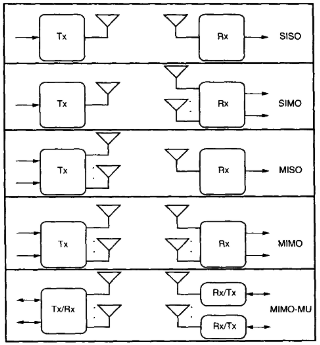
\includegraphics [width=0.6\textwidth]{./figure/mimo.png}
    \caption{无线通信中的天线配置方式}
    \label{fig:mimo}}
\end{figure}


\end{spacing}

%%%%%%%%%%%%
%  参考文献
%%%%%
% \small
\bibliographystyle{gbt7714-2005}
\bibliography{ref}
% \small
% \begin{thebibliography}{99}
% \setlength{\parskip}{0pt}  %段落之间的竖直距离
% \bibitem{1}李姗泽.学前教育应重视中华民族优秀传统文化——论民间游戏在幼儿园课程资源中的地位和作用[J].课程.教材.教法,2005(05):31-35.

% \end{thebibliography}

\end{document}
